%%%%%%%%%%%%%%%%%%%%%%%%%%%%%%%%%%%%%%%%%
% Beamer Presentation
% LaTeX Template
% Version 1.0 (10/11/12)
%
% This template has been downloaded from:
% http://www.LaTeXTemplates.com
%
% License:
% CC BY-NC-SA 3.0 (http://creativecommons.org/licenses/by-nc-sa/3.0/)
%
%%%%%%%%%%%%%%%%%%%%%%%%%%%%%%%%%%%%%%%%%

%----------------------------------------------------------------------------------------
%	PACKAGES AND THEMES
%----------------------------------------------------------------------------------------

\documentclass[UTF8,aspectratio=169,14pt]{ctexbeamer}

\usepackage{hyperref}
\hypersetup{
	colorlinks=true,
	linkcolor=red,
	anchorcolor=blue,
	citecolor=green
}

\mode<presentation> {
	
	% The Beamer class comes with a number of default slide themes
	% which change the colors and layouts of slides. Below this is a list
	% of all the themes, uncomment each in turn to see what they look like.
	
	%\usetheme{default}
	%\usetheme{AnnArbor}
	%\usetheme{Antibes}
	%\usetheme{Bergen}
	%\usetheme{Berkeley}
	%\usetheme{Berlin}
	%\usetheme{Boadilla}
	%\usetheme{CambridgeUS}
	%\usetheme{Copenhagen}
	%\usetheme{Darmstadt}
	%\usetheme{Dresden}
	%\usetheme{Frankfurt}
	%\usetheme{Goettingen}
	%\usetheme{Hannover}
	%\usetheme{Ilmenau}
	%\usetheme{JuanLesPins}
	%\usetheme{Luebeck}
	\usetheme{Madrid}
	%\usetheme{Malmoe}
	%\usetheme{Marburg}
	%\usetheme{Montpellier}
	%\usetheme{PaloAlto}
	%\usetheme{Pittsburgh}
	%\usetheme{Rochester}
	%\usetheme{Singapore}
	%\usetheme{Szeged}
	%\usetheme{Warsaw}
	
	% As well as themes, the Beamer class has a number of color themes
	% for any slide theme. Uncomment each of these in turn to see how it
	% changes the colors of your current slide theme.
	
	%\usecolortheme{albatross}
	%\usecolortheme{beaver}
	%\usecolortheme{beetle}
	%\usecolortheme{crane}
	%\usecolortheme{dolphin}
	%\usecolortheme{dove}
	%\usecolortheme{fly}
	%\usecolortheme{lily}
	%\usecolortheme{orchid}
	%\usecolortheme{rose}
	%\usecolortheme{seagull}
	%\usecolortheme{seahorse}
	%\usecolortheme{whale}
	%\usecolortheme{wolverine}
	
	%\setbeamertemplate{footline} % To remove the footer line in all slides uncomment this line
	%\setbeamertemplate{footline}[page number] % To replace the footer line in all slides with a simple slide count uncomment this line
	
	%\setbeamertemplate{navigation symbols}{} % To remove the navigation symbols from the bottom of all slides uncomment this line
}

\usepackage{graphicx} % Allows including images
\graphicspath{{./figs/}}
\usepackage{booktabs} % Allows the use of \toprule, \midrule and \bottomrule in tables
\usepackage{longtable}
\usepackage{listings}
\usepackage{xcolor}
\lstset{numbers=left, %设置行号位置
	numberstyle=\tiny, %设置行号大小
	keywordstyle=\color{blue}, %设置关键字颜色
	commentstyle=\color[cmyk]{1,0,1,0}, %设置注释颜色
	frame=single, %设置边框格式
	escapeinside=``, %逃逸字符(1左面的键),用于显示中文
	%breaklines, %自动折行
	extendedchars=false, %解决代码跨页时,章节标题,页眉等汉字不显示的问题
	xleftmargin=2em,xrightmargin=2em, aboveskip=1em, %设置边距
	tabsize=4, %设置tab空格数
	showspaces=false %不显示空格
}
% Fonts
% \usepackage{libertine}
% \setmonofont{Courier}
\setCJKsansfont[ItalicFont=Noto Serif CJK SC Black, BoldFont=Noto Sans CJK SC Black]{Noto Sans CJK SC}


%----------------------------------------------------------------------------------------
% TITLE PAGE
%----------------------------------------------------------------------------------------

\title[第21讲]{第二十一讲 :异步编程(Asynchronous Programming)} % The short title appears at the bottom of every slide, the full title is only on the title page
\subtitle{第4节:Self-Referential Structs \& Pin}
\author{向勇、陈渝} % Your name
\institute[清华大学] % Your institution as it will appear on the bottom of every slide, may be shorthand to save space
{
  清华大学计算机系 \\ % Your institution for the title page
  \medskip
  \textit{xyong,yuchen@tsinghua.edu.cn} % Your email address
}
\date{\today} % Date, can be changed to a custom date

\begin{document}

\begin{frame}
\titlepage % Print the title page as the first slide
\end{frame}

%----------------------------------------------
\begin{frame}
\frametitle{提纲} % Table of contents slide, comment this block out to remove it
\tableofcontents % Throughout your presentation, if you choose to use \section{} and \subsection{} commands, these will automatically be printed on this slide as an overview of your presentation

%% itemize
Ref:
    \begin{itemize}
        \item \href{}{xxxx}
    \end{itemize}

\end{frame}
%----------------------------------------------
%%  PRESENTATION SLIDES
%----------------------------------------------
\section{第4节:Self-Referential Structs \& Pin} % Sections can be created in order to organize your presentation into discrete blocks, all sections and subsections are automatically printed in the table of contents as an overview of the talk
%----------------------------------------------
\subsection{xxxx} % A subsection can be created just before a set of slides with a common theme to further break down your presentation into chunks
%----------------------------------------------
\begin{frame}[fragile]
    \frametitle{Self-Referential Structs}
%    \framesubtitle{xxxx}
% ### 21.4 Self-Referential Structs & Pin
% 
% Ref: https://cfsamson.github.io/books-futures-explained/4_pin.html#pin
% 
% #### Self-Referential Structs
% 
% Ref: https://os.phil-opp.com/async-await/#self-referential-structs
% 
\begin{block}{}
    \begin{verbatim}
    //rust code
    async fn pin_example() -> i32 {
        let array = [1, 2, 3];
        let element = &array[2];
        async_write_file("foo.txt", element.to_string()).await;
        *element
    }
    \end{verbatim}
\end{block}
% 
The struct for the "waiting on write" state

\begin{block}{}
    \begin{verbatim}
    //rust code
    struct WaitingOnWriteState {
        array: [1, 2, 3],
        element: 0x1001c, // address of the last array element
    }
    \end{verbatim}
\end{block}
% 
\end{frame}
%----------------------------------------------
\begin{frame}[fragile]
    \frametitle{The Problem with Self-Referential Structs}
%    \framesubtitle{xxxx}
% #### The Problem with Self-Referential Structs
% 
% Ref: https://os.phil-opp.com/async-await/#the-problem-with-self-referential-structs
% 
{\color{red}memory layout of self-referential struct}
% 
%% figure
    \begin{figure}
    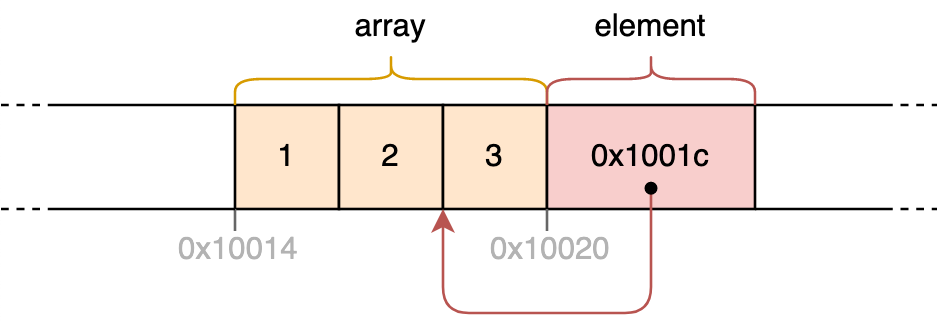
\includegraphics[width=0.8\linewidth]{figs/self-referential-struct.png}
%    \caption{xxxx}
    \end{figure}
% ![self-referential-struct](figs/self-referential-struct.svg)
% 
{\color{red}After moving this struct to a different memory address}
% 
%% figure
    \begin{figure}
    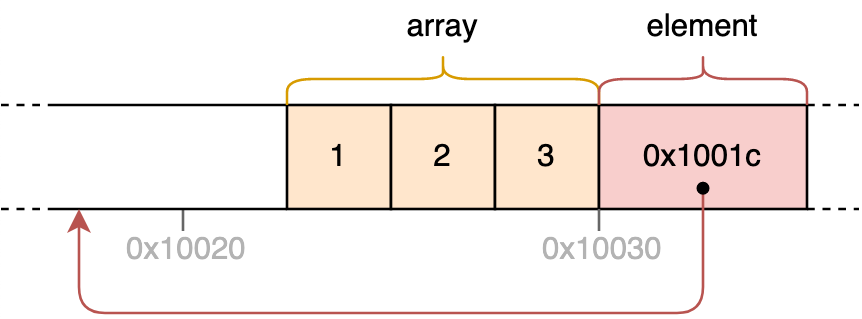
\includegraphics[width=0.8\linewidth]{figs/self-referential-struct-moved.png}
%    \caption{xxxx}
    \end{figure}
% ![self-referential-struct-moved](figs/self-referential-struct-moved.svg)
% 
\end{frame}
%----------------------------------------------
\begin{frame}[fragile]
    \frametitle{Possible approaches to solve the dangling pointer problem}
%    \framesubtitle{xxxx}
% #### Possible approaches to solve the dangling pointer problem
% 
% Ref: https://os.phil-opp.com/async-await/#possible-solutions
% 
%% itemize
    \begin{itemize}
        \item {\color{red}Update the pointer on move:} Require extensive changes to Rust that would result in potentially huge  performance losses.
        \item {\color{red}Store an offset instead of self-references:}: Require the compiler to {\color{red}detect all self-references} or need a runtime system again to analyze references and correctly create the  state structs.
        \item {\color{red}Forbid moving the struct:} This approach can be implemented at the type system level without additional  runtime costs
    	\begin{itemize}
    	    \item It puts the burden of dealing with  move operations on possibly self-referential structs on the programmer
    	\end{itemize}
    \end{itemize}

\end{frame}
%----------------------------------------------
\begin{frame}[fragile]
    \frametitle{Defination of Pin}
%    \framesubtitle{xxxx}
% #### Defination of Pin
% 
% Ref: https://cfsamson.github.io/books-futures-explained/4_pin.html#definitions
% https://github.com/rust-lang/rfcs/blob/master/text/2349-pin.md
% the pinning API was proposed in RFC 2349
% 
%% itemize
    \begin{itemize}
        \item Pin wraps a pointer. A reference to an object is a pointer
    	\begin{itemize}
    	    \item {\color{red}Reference type}. In order to break apart a large future into its smaller components, and put  an entire resulting future into some immovable location, we need a reference type for methods like `poll`
    	\end{itemize}
        \item Pin gives some guarantees about the *pointee* (the data it points to)
    	\begin{itemize}
    	    \item {\color{red}Never to move before being dropped}. To store references into itself, we decree that by the time you initially `poll`, and promise to never move an immobile future again
    	\end{itemize}
    \end{itemize}
% 
\begin{block}{}
    \begin{verbatim}
    //rust code
trait Future {
    type Item;
    type Error;

    fn poll(self: Pin<Self>, cx: &mut task::Context) -> Poll<Self::Item, Self::Error>;
}
        \end{verbatim}
\end{block}
% 
\end{frame}
%----------------------------------------------
\begin{frame}[fragile]
    \frametitle{Pinning to the heap}
%    \framesubtitle{xxxx}
% #### Pinning to the heap
% 
% Ref: https://cfsamson.github.io/books-futures-explained/4_pin.html#pinning-to-the-heap
% 
Pinning to the heap is safe so the user doesn't need to implement any unsafe code.
% 
%% itemize
    \begin{itemize}
        \item Once the data is allocated on the heap it will have a stable address
        \item Examp: \href{https://cfsamson.github.io/books-futures-explained/4_pin.html#pinning-to-the-heap}{Pinning to the heap}
    \end{itemize}

\end{frame}
%----------------------------------------------
\end{document}
